There is no established standard of characterisation measurements for granular materials. Typical measurements include heap test, rotating drum test, linear/ring shear cell test, and the silo flow test..., in which the output is the bulk parameter, which defines how the granular material behaves in large quantity~-~such as the angle of repose (AoR), shear stress, flow rate. 

This research is focused on one of the essential bulk parameters to describe the characteristics of the granular materials~-~the static angle of repose. Static AoR, described in Fig.~\ref{fig:StaticAoR}, is defined as the angle that granular solids form when it is piled with a flat surface and is essential to characterise the coarseness and smoothness of materials. This, in turn, can help design a process involved with the material~-~lower static AoR implies more flowable and thus easier to transport with less energy~\cite{TEFERRA201945}.


\begin{figure}[H]
    \centering
    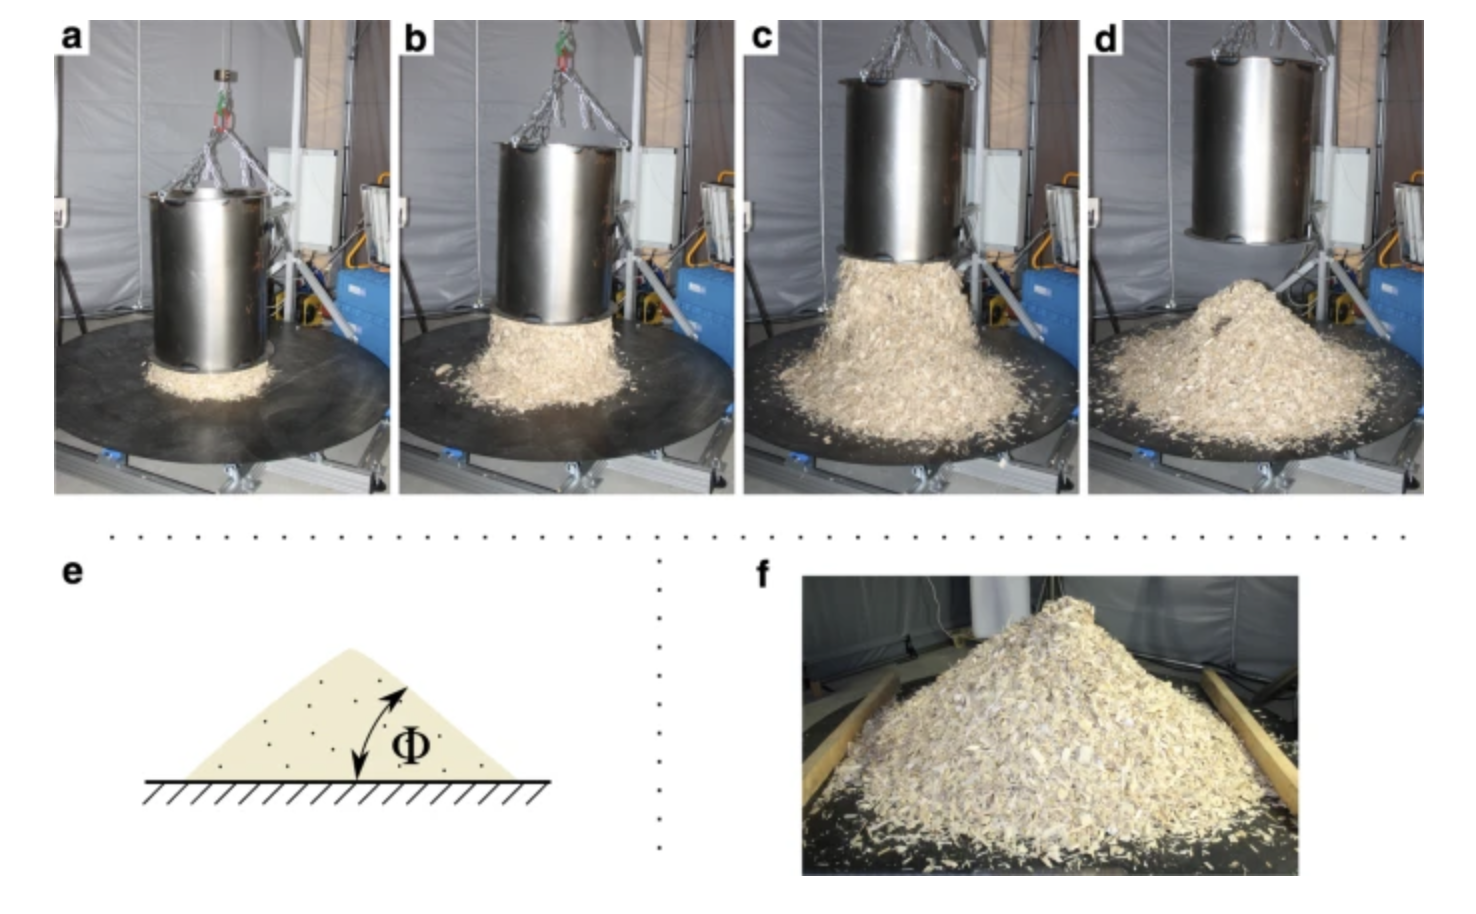
\includegraphics[scale=0.5]{StaticAoR.png}
    \caption{Static Angle of Repose measurement steps~\cite{Rackl:2018te}.}\label{fig:StaticAoR}
\end{figure}


